\chapter{EVO Protocol }\label{sec:evoprotocol}


\section{The Manifold System}

There are two distinct concepts used throughout this paper:
\begin{itemize}
	\item Manifolds
	\item evo
\end{itemize}

\label{Manifolds}Manifolds compromise the mechanisms that enforce the protocol in such a way that it enables composable extensions to be utilized. 

\section{Manifolds}\label{sec:manifolds}
EVO, short for \texttt{embedded volumetric optionality} represents a derived utility token that is minted only when deposits are made into the corresponding \texttt{manifold} contract for that underlying instrument. 

EVO tokens are minted and burned on-demand by deposit and withdraw operations directly on the contract.\linebreak

\begin{tcolorbox}
	EVO tokens do not imply the same epoch from asset to asset, nor should you infer that the same properties that are found in GasEVO would be found in another EVO-type token/instrument
\end{tcolorbox}


\subsection{Contract Operations}

There are three primary operations that will affect the \texttt{transfer rate}

\begin{itemize}
	\item Deposits
	\item Withdrawals 
	\item Transfers
\end{itemize}


These three operations, deposit, withdraw and transfer,  can all equally contribute to
the \texttt{transfer rates} that are tracked totally and individually per account. The \texttt{business logic} is stored for a defined set of time. \textbf{GasEVO} implements a 25 day epoch. We would like to reiterate that this parameter was tested through simulations and not chosen arbitrarily. 

\subsection{Token Mechanics}
The token price is determined dynamically and individually for each holder. This is based on the
information stored and/or updated in the smart contract during previous transactions. 

SHALL use$ evo$ to reference ONLY the minted asset created upon deposits.
\linebreak

\begin{itemize}
	\item $evo$ MUST ONLY reference minted assets created upon deposits at the defined minting ratio (e.g. 1:1).
	\item $ml$ MUST ONLY referenced the governance and utility interface contract that administers the protocol as a whole
\end{itemize}

SHALL use  manifold  or $ml$ to reference ONLY the protocol utility token.

\newpage
\subsection{Price for Individual Account} 
All three operations such as deposit, withdraw and transfer can equally contribute to the transfer rates that are tracked totally and individually (as per holder)
by the smart contract for the period of the last 25 days. The token price is determined dynamically (and individually for each holder) based on the information stored or updated in the smart contract during previous transactions:

\begin{tcolorbox}
	\label{eq:Base Primitive Equation}
	
	
	\begin{equation}
		P_{t+1}(h, a):=\sqrt{\frac{D_{t}}{S_{t}}}+I_{t+1}^{\prime}(h, a)
	\end{equation}
	
\end{tcolorbox}

The above equation will compute the price for a holder $h$ to purchase
certain amount a of EVO tokens in exchange for a base deposit in the underlying instrument (ETH) at the given discrete time-point {t + 1}\footnote{(Equivalently a transaction
number}, where $Dt$ stands for the deposit of ETH in the smart contract at previous time-point.

\begin{itemize}
	\item $Dt$
\end{itemize}


\label{total.supply.minted-evo}
$St$ stands for the total supply of EVO tokens so far

\label{deposits.discrete}
$Dt$  stands for deposits at a point in time 
\newline
\label{total.supply.so-far}
$S_t$ = Total Supply So Far

\begin{equation}
	I_{t+1}^{\prime}(h, a)
\end{equation}

\newpage

\subsection{Proportional Ratio for Discounted Interest Rate Growth}
discounted interest and it can grow proportionally to a within
a range of [0,0.24] of $a$

\label{discounted.interest.range}
\begin{equation}
	[0,0.24] \text{of $a$ }
\end{equation}

\subsection{Calculate Individual Account Transference}
How much an individual account has transferred over the last 25 days 

\label{total.individual.avg.transfer.rate}
\begin{equation}
	\begin{eqfloat}
		\operatorname{avg}\left(R_{t+1}(h, a)\right):=\operatorname{avg}\left(R_{t}(h)\right)+a
		\caption{Total Avg. Transfer Rate for Individual Account}
	\end{eqfloat}
\end{equation}

\begin{tcolorbox}
	\subsection{The Total Daily Average Transfer Rate for all holders }
	\label{total.aggregate.daily.avg.transfer.rate}
	\begin{equation}
		\operatorname{avg}\left(\bar{R}_{t+1}(h, a)\right):=\operatorname{avg}\left(\bar{R}_{t}(h)\right)+a
	\end{equation}
\end{tcolorbox}

\begin{tcolorbox}
	\subsection{ Future Transfer Ratio }
	\begin{equation}
		\tau=\frac{\operatorname{avg}\left(R_{t+1}(h, a)\right)}{\operatorname{avg}\left(\bar{R}_{t+1}(h, a)\right)}
	\end{equation}
\end{tcolorbox}

\begin{tcolorbox}
	\subsection{ Ownership Ratio By an Account in a previous point of time }
	\begin{equation}
		\theta=\frac{B_{t}(h)}{S_{t}}
	\end{equation}
\end{tcolorbox}

\begin{tcolorbox}
	\label{Interest Rate}
	\begin{equation}
		I_{t+1}(h, a):=\frac{a \times \min (\operatorname{avg}(\beta, \tau), m)}{100}
	\end{equation}
\end{tcolorbox}

\begin{tcolorbox}
	\subsection{Discounted Interest Rate}
	\label{Discounted Interest Rate}
	\begin{equation}
		I_{t+1}^{\prime}(h, a):=\max \left(I_{t+1}(h, a), l_{t+1}^{\prime}(h, a)\right)-l_{t+1}^{\prime}(h, a)
	\end{equation}
\end{tcolorbox}


\begin{tcolorbox}
	\subsection{Normalized Interest Rate}
	\label{Normalized Interest Rate }
	\begin{equation}
		l_{t+1}^{\prime}(h, a):=\frac{a \times \sqrt{l * \max \left(\min \left(\theta, l^{2}\right), 1\right)}}{100}
	\end{equation}
\end{tcolorbox}



\newpage


\section{Protocol Context}

Manifolds and $evo$ tokens represent the two distinct parameters at plat in the protocol. Manifolds are the constructed routing and logic that is said to be embedded  within, with $evo$ tokens the created asset representing a claim on the depository contract within that specific manifold. 
This paper primarily deals with $evo$ tokens: a forthcoming paper detailing additional extensions such as adversarial exchange further extends the manifold concept.


\subsection{Manifolds}
We define a Manifold as the  potential difference between the underlying asset $Ua$ and the forward contract of that asset $Fa$. The manifold is a conduit in which fully collateralize backing is unnecessary due to the design of the volumetric comptroller. \footnote{}

\subsection{Advantages over current protocols}

Compound Finance for example illustrates the issue with {illiquid assets}. 

\begin{quote}
	Generally, large or liquid assets have high collateral factors, while small or illiquid assets have low collateral factors. If an asset has a 0per-cent collateral factor, it can't be used as collateral (or seized in liquidation), though it can still be borrowed.\footnote{see compound finance whitepaper, https://compound.finance/documents/Compound.Whitepaper.pdf}
\end{quote}

Utilizing a \textbf{manifold} for such non-liquid assets would enable the $ evo $ derived underlying asset additional market access to such existing protocols. We should note that this does not materially change the underlying market issues with the asset, only that their is now programmatic guardrails to minimize potential contagion / knockdown affects arising from usage of less liquid  assets.




\section{Architecture}
\label{architecture}

An ERC20 smart contract will contain the information about the balance of every address.
Floating point math is provided by the excellent library \textt{ABDK libraries-solidity}\footnote{https://github.com/abdk-consulting/abdk-libraries-solidity/blob/ABDKMath64x64.sol at hash: 16d7e1dd8628dfa2f88d5dadab731df7ada70bdd }

See the \textbf{DEVELOPMENT.md} file in the GitHub.com repository.

\subsection{Requirements Overview}

An implementation of the EVO protocol and its manifold constructs.

\subsection{Protocol Specification}
The above equation will compute the price for a holder $h$ to purchase a certain amount of `EVO` tokens in exchange for a base deposit in ETH at point in time  $t +1$ \neweline $Dt$ stands for the deposit of ETH in the smart contract at previous time - point
\newline$St$
    
stands for the total supply of the minted asset \texttt{EVO-} tokens so far.

\subsection{Base Ratio}
The first component with the token - base ratio\neweline $ Dt/St $ under the square root is the *indicative price* and \textbf{does not depend on the purchase/transferred} amount, $a$

\subsection{Discounted Interest Rate}
\begin{equation}
	I_{t+1}^{\prime}(h, a)
\end{equation}

This component is called the *discounted interest rate* and it can grow *proportionally* to a within a range of 
\begin{equation}
	[0, 0.24] a 
\end{equation}
.
Higher interest payouts can slow down, \textbf{decelerate}, the price movement. 

The Interest Rate \ref{Interest Rate} determines the speed, in essence the \textbf{acceleration}, such price can change depending on the market demand and supply pressure for EVO-derived tokens.

Interest is computed individually for each EVO holder. \footnote{
*Note* that all interest payments are contributed to the same common deposit $Dt$ on the smart contract, which is supporting the indicative price. This means that interest is shared by all holders that *choose not to trade their tokens* at the moment.}




\label{sec:Calculations}
\subsection{Address Information}
Address Information


\begin{equation}
	B(h) s.t. Bt + 1(h, a): = Bt(h) + a 
\end{equation}


In addition to the individual balances, EVO contract keeps track about how much each holder has transferred in the last defined epoch \footnote{an epoch as defined in the GasEVO implementation as 25 days. Epochs may be customized and should generally be in multiples of 6}

\label{sec:Calculations}
\subsection{Total average transfer rate for an address}

\begin{equation}
	avg(Rt + 1(h, a)): = avg(Rt(h)) + a
\end{equation}


\label{sec:Calculations}
\subsection{Total average daily transfer rate for all holders}
\begin{equation}
	avg(R¯ t + 1(h, a)): = avg(R¯t(h)) + a
\end{equation}

\subsection{Calculations Example}
More formally calculation of the individual interest rate as well as the applied ownership discount can be described in following steps:

For: l := 4 , m := 26 are the \url{ManifoldBottom} and \url{Manifold-Top} transfer rate constants and \footnote{ManifoldBottom and ManifoldTop are defined parameters and can be changed}

\label{sec:Calculations}
\begin{equation}
	\beta=\frac{\operatorname{avg}\left(B_{t+1}(h, a)\right)}{S_{t+1}}, 
\end{equation}
\newpage
\section{Future Balance Ratio}
For the \textit{future balance ratio}, we resolve
\label{sec:Calculations}
\begin{equation}
	\beta=\frac{\operatorname{avg}\left(B_{t+1}(h, a)\right)}{S_{t+1}}
\end{equation}
\label{future transfer ratio}
\subsection{Future transfer ratio}
\begin{equation}
	\tau=\frac{\operatorname{avg}\left(R_{t+1}(h, a)\right)}{\operatorname{avg}\left(\bar{R}_{t+1}(h, a)\right)}
\end{equation}

\subsection{Ownership Ratio at a previous point in time
	\begin{equation}
		\theta=\frac{B_{t}(h)}{S_{t}}
	\end{equation}
	
	\subsection{Calculated Interest Rate}
	\begin{equation}
		I_{t+1}(h, a):=\frac{a \times \min (\operatorname{avg}(\beta, \tau), m)}{100}
	\end{equation}
	The calculated potential daily transfer rate  is the ownership ratio at a *discrete point in `block time`. Then we resolve the \textit{interest rate}
	
	\subsection{Discounted Interest Rate}
	\begin{equation}
		l_{t+1}^{\prime}(h, a):=\frac{a \times \sqrt{l * m a x\left(\min \left(\theta, l^{2}\right), 1\right)}}{100}
	\end{equation}
	
	
	\begin{equation}
		P_{t+1}(h, a):=\sqrt{\frac{D_{t}}{S_{t}}}+I_{t+1}^{\prime}(h, a)
	\end{equation}
	
	
	\label{Discounted Interest Rate}
	\subsection{Discounted Interest Rate}
	\begin{equation}
		P_{t+1}(h, a):=\sqrt{\frac{D_{t}}{S_{t}}}+I_{t+1}^{\prime}(h, a)\footnote{Bounded by $O[sqrt(n)]$}
	\end{equation}
	\ref{primitive rate}
	
	
	\label{Ownership Ratio for the Discounted Interest Rate}
	\subsection{Ownership Ratio for Discounted Rate}
	
	We can then derive the ownership ratio for discount by
	\begin{equation}
		l_{t+1}^{\prime}(h, a):=\frac{a \times \sqrt{l * \max \left(\min \left(\theta, l^{2}\right), 1\right)}}{100}
	\end{equation}
	
	whereas 1 per-cent` is the {discount}, thereby computing the \texttt{discounted interest} as
	
	\begin{equation}
		I_{t+1}^{\prime}(h, a):=\max \left(I_{t+1}(h, a), l_{t+1}^{\prime}(h, a)\right)-l_{t+1}^{\prime}(h, a)
	\end{equation}
	
	
	Price dynamics of equation (1) depends on the transactions volume conducted by all of the involved market participants and bounded by $ O(sqrt(n)) $.
	
	Therefore it can be expected that the demand for EVO Protocol based tokens like GasEVO will be able to approximate future market sentiment for the value of the underlying asset, whereas GasEVO may be seen as an approximation of the value of storage as a function of the underlying asset, Ethereum.\footnote{ (i.e. gwei, or as a fixed unit of account for contracting)}
	\end{flushleft} 
	\newpage
	
	
	
	\chapter{Manifolds}
	
	
	\begin{quote}
		The new capitalist axiomatic: a mirror of velocity.
	\end{quote}
	
	
	\section{Implementation Benchmark}
	
	\subsection{Uniform Cost Search}
	Uniform cost search expands the node with the lowest cost-so-far 
	$\sum{i j}_{i j} c_{i j}$ on the fringe. Hence, the relative ordering between two nodes is determined by the value of \sum${i j} c_{i j}$ for a given node. So only for \mathcal{$d_{i j}=\alpha c_{i j}, \alpha>0,$ can we conclude, $\sum_{i j in \text { path }(n)} d_{i j} \geq \sum_{i j in \text { path }(m)} d_{i j} \Longleftrightarrow \sum_{i j in \operatorname{path}(n)} c_{i j} \geq \sum_{i j in \operatorname{path}(m)}$ $c_{i j},$} for some nodes $n$ and $m$ $ $
	
	\subsection{Iterative Search Parameters}
	
	Cost of $X$ $+$ $Y$ is decreased by $n$, $n$ > $0$, the edge is not on the optimal path, and was not explored by
	the first search.
	
	
	
	\newpage
	
	\chapter{Volumetric Manifolds}
	
	> A constructed mechanism for facilitation of efficient and effective contract$^[1]$ trading 
	
	$
	G:=(V, E, w)
	$
	
	
	
	weighted by the function $w: E \rightarrow \mathbb{R}^{+}$ corresponding to the price of some trade $e \in E$
	
	
	$ V,|V| \leq|\mathbb{N}| $
	
	
	
	Consider an abstract liquid trading (ALT) system as a weighted directed graph $G:=(V, E, w),$ where set of vertices $V,|V| \leq|\mathbb{N}|$ contains digital representation of all trade-able assets in $G,$ set of edges $E=\{e \in V \times V:$ $w(e)>0\}$ represents all possible atomic $^{79}$ asymmetric $^{80}$ trades, which are weighted by the function $w: E \rightarrow \mathbb{R}^{+}$ corresponding to the price of some trade $e \in E$
	
	
	\subsection{Liquidity Point/Vertex}
	
	$
	\text { Any liquid vertex } v \in V \text{ has both } d e g^{-}(v) \geq 1 \text{ and } \operatorname{deg}^{+}(v) \geq 1
	$
	
	
	Liquidity Indifference Preference Paths$^{2}$
	
	$C_{B}(v):=\sum_{s \neq t \neq v \in V} \frac{\sigma_{s t}(v)}{\sigma_{s t}}: \forall(s, t) \in S, \text{ where } \sigma_{s t}:=\sum_{(s, t) \in S} \sum_{e \in(s, t)} w(e)$
	
	
	\subsection{Ownership Ratio at a discrete point in block time
		is the \label{Ownership Ratio at a discrete point in block time and
			\begin{equation}
				\theta=\frac{B_{t}(h)}{S_{t}}
			\end{equation}
			
			
			Vertex $v \in V$ represents half-liquid asset  when either $\operatorname{deg}^{-}(v)=0$ (source) $\operatorname{or} \operatorname{deg}^{+}(v)=0(\operatorname{sink}),$ where $\operatorname{deg}^{(-1+)}: V \rightarrow \mathbb{N}$ is respectively a number
			of tail ends (indegree) and a number of head ends (outdegree) from vertices adjacent to $v$.
			
			\
			\subsection{Liquidity Preference Path}
			
			Let $S \subset V \times V$ contain all shortest paths from vertex $s$ to vertex $t: \forall s, t \in V$ Also let vertex $v \in V$ have the maximal $^{82}$ betweenness centrality measure $C_{B}(v):=\sum_{s \neq t \neq v \in V} \frac{\sigma_{s t}(v)}{\sigma_{s t}}: \forall(s, t) \in S,$ where $\sigma_{s t}:=\sum_{(s, t) \in S} \sum_{e \in(s, t)} w(e)$
			and $\sigma_{s t}(v)$ 
			is a sum of only those shortest paths in $S$ which contain $v .$ We say that $(s, t) \in S$ **is a path with preferable liquidity if it ends with** 
			
			$v$ `in essence,` $t=v$
			
			So that we may compute the approximate list of *preferable assets*, we highlight two distinct properties that are both necessary and sufficient.
			
			In order to capture a desired hyper-manifold liquidity property of an always preferable asset, $G,$ , we identify such asset not only as a preferable "exit" (that is to say, the position can be unwound within a reasonable amount of blocks without materially affecting price of the asset) $vertex$, but also as the one that can be consequently traded for any other liquid asset in $G$ at the most best settlement price.
			
			
			\paragraph{List}
			
			$(\operatorname{manifold})$
			$(\operatorname{hyper-manifold})$
			$(\operatorname{supra-manifold})$
			$(\operatorname{inter-manifold})$
			
			
			Let $S \subset V \times V$ contain all shortest paths from vertex $s$ to vertex $t: \forall s, t \in V$ Also let vertex $v \in V$ have the maximal $^{82}$ betweenness centrality measure $C_{B}(v):=\sum_{s \neq t \neq v \in V} \frac{\sigma_{s t}(v)}{\sigma_{s t}}: \forall(s, t) \in S,$ where $\sigma_{s t}:=\sum_{(s, t) \in S} \sum_{e \in(s, t)} w(e)$
			
			
			and $\sigma_{s t}(v)$ is a sum of only those shortest paths in $S$ which contain $v .$
			
			We say that $(s, t) \in S$ is a path with **preferable liquidity** if it ends with $v,$ i.e. $t=v$
			
			
			In order to capture a desired liquidity preference curve ("hyper manifold") property of an always preferable asset in an 
			"ALT"-system $G,$ we must first identify such asset. Such an asset must exhibit the properties of not only having *genuine* liquidity (that is to say, "a preferable "exit" $(\operatorname{sink})$ vertex"), but also as the one that can be consequently traded for any other liquid asset in $G$ at the most attractive price.
			
			\subsection{Flash Loan led path-finding}
			
			A "liquid"$^[3]$ vertex $v \in V\left(G^{\prime}\right)$ of a complete liquid subgraph $G^{\prime} \subseteq G$ is called a *hyper*-liquid vertex when any preferable liquidity path 
			
			$p=(s, v)$ 
			
			can be almost surely continued with an efficient trade for any other liquid $u \in V\left(G^{\prime}\right), u \neq v$ in such a way that $\sum_{e \in(s, u)} w(e) \leq \sum_{e \in(s, v)} w(e)+\sum_{e \in(v, u)} w(e)$ and $(s, u)$ is
			a shortest path.
			
			
			\subsection{Informative}
			
			$^[1]$ Contracts meaning *Smart Contracts*
			
			$^[3]$ Pockets of Liquidity is a well known microstructure in markets. Further research in the microstructural differences between AMM's and traditional settlement procedures (e.g. LMM, FIFO, etc) must be pursued.
			
			
			
			\newpage
			
			\section{References}
			
			GFI. 2015. GFI Swaps Exchange LLC rulebook. GFI Technical Report.
			\footnote{https://www.cftc.gov/sites/default/files/stellent/groups/public/@otherif/
			documents/ifdocs/exhibitm1rulebookgfiswaps.pdf}
			
			
			Pavan, A., I. Segal, and J. Toikka. 2014. Dynamic mechanism design: A Myersonian approach.
			Econometrica 82:601–53.
			
			Protter, P. 2005. Stochastic integration and differential equations, second edition. Heidelberg:
			Springer.
			
			Rostek, M., and M. Weretka. 2012. Price inference in small markets. Econometrica 80:687–711.
			2015. Dynamic thin markets. Review of Financial Studies 28:2946–92.
			
			
			Ye, L. 2016. Understanding the impacts of dark pools on price discovery. Working paper, The
			Chinese University of Hong Kong, Shenzhen. https://arxiv.org/pdf/1612.08486.pdf.
			
			"A Liquidity Based Model of Security Design" (with Peter DeMarzo), Econometrica 1999, Volume 67: 65-99.\footnote{The copyright to this article is held by the Econometric Society, http://www.econometricsociety.org.}
			
			"Optimal Innovation of Futures Contracts" (with Matthew O. Jackson), Review of Financial Studies 
			1989, Volume 2: 275-296.
			
			\newpage
			
			\chapter{Appendix}
			
			\begin{itemize}
				\item Q3 2020
				\item Q4 2020
				\item Q1 2021
			\end{itemize}
			
			
			
			\section{Reference Equations}
			
			
			$
			s_{\text {minted}}=\frac{x_{\text {deposited}}}{x_{\text {starting}}} \cdot s_{\text {starting}}
			$
			
			\subsection{Fees}
			$
			f_{1,2}=1-\frac{\sqrt{k_{1}}}{\sqrt{k_{2}}}
			$
			
			
			
			\subsection{Manifold Exchange}
			\begin{equation}
				P_{t+1}(h, a):=\sqrt{\frac{D_{t}}{S_{t}}}+I_{t+1}^{\prime}(h, a)
			\end{equation}
			
			\text{https://github.com/abdk-consulting/abdk-libraries-solidity/commit/16d7e1dd8628dfa2f88d5dadab731df7ada70bdd}
			
			\subsection{Manifold Interest Rate}
			\begin{equation}
				I_{t+1}^{\prime}(h, a):=\max \left(I_{t+1}(h, a), l_{t+1}^{\prime}(h, a)\right)-l_{t+1}^{\prime}(h, a)
			\end{equation}
			
			\begin{equation}
				I_{t+1}^{\prime}(h, a) \in[0,0.24]
			\end{equation}
			The amount $a$ as restricted by the constants and the formula construct defined as \ref{Base Primitive Equation}base primitive equation will reflect accurately.
			
			\section{Lists}\label{sec:lists}
			Three types of list-environments are commonly used: \texttt{itemize}, \texttt{enumerate}, and \texttt{description}. The following example uses \texttt{itemize} to create a list without numbering
			\begin{itemize}
				\item point one; and
				\item point two
			\end{itemize}
			created using
			\begin{verbatim}
\begin{itemize}
  \item point one; and
  \item point two
\end{itemize}
			\end{verbatim}
			
			The following example uses \texttt{enumerate} to create a list with numbering
			\begin{enumerate}
				\item point one; and
				\item point two
			\end{enumerate}
			created using
			\begin{verbatim}
\begin{enumerate}
  \item point one; and
  \item point two
\end{enumerate}
			\end{verbatim}
			
			The following example uses \texttt{description} to create a list with custom text as bullet-points
			\begin{description}
				\item[P1] point one; and
				\item[P2] point two
			\end{description}
			created using
			\begin{verbatim}
\begin{description}
  \item[P1] point one; and
  \item[P2] point two
\end{description}
			\end{verbatim}
			
			
			\section{Tables}\label{sec:tables}
			Table~\ref{tab:table} shows an example of a simple table-layout. Try to avoid vertical lines on tables. The Internet contains countless resources on how to create special elements and structures in tables such as cells spanning multiple rows, rotated text, sideways tables, justification of cell elements, etc.
			\begin{table}[ht]
				\begin{center}
					\caption{Driving cycle data of ECE-15, EUDC, and NEDC.}\vspace{1ex}
					\label{tab:table}
					\begin{tabular}{llccc}\hline
						Description      & Unit & ECE   & EUDC  & NEDC   \\ \hline
						Duration         & s    & 780   & 400   & 1180   \\
						Distance         & km   & 4.052 & 6.955 & 11.007 \\
						Average velocity & km/h & 18.7  & 62.6  & 33.6   \\
						Idle speed       & \%   & 36    & 10    & 27     \\ \hline
					\end{tabular}
				\end{center}
			\end{table}
			
			This table was created using
			\begin{verbatim}
\begin{table}[ht]
\begin{center}
\caption{Driving cycle data of ECE-15, EUDC, and NEDC.}\vspace{1ex}
\label{tab:table}
\begin{tabular}{llccc}\hline
Description & Unit & ECE & EUDC & NEDC \\ \hline
Duration & s & 780 & 400 & 1180 \\
Distance & km & 4.052 & 6.955 & 11.007 \\
Average velocity & km/h & 18.7 &  62.6 & 33.6 \\
Idle speed & \% & 36 & 10 & 27 \\ \hline
\end{tabular}
\end{center}
\end{table}
			\end{verbatim}
			Table~\ref{tab:table_advanced} shows a more advanced version of Tab.~\ref{tab:table} using the \texttt{booktabs} package. Inspect the source code of this document to see how this was done.
			\begin{table}[ht]
				\begin{center}
					\small
					\caption{Driving cycle data of ECE-15, EUDC, and NEDC.}\vspace{1ex}
					\label{tab:table_advanced}
					\begin{tabular}{@{}lcccc@{}}\toprule[1.5pt]
						& & \multicolumn{3}{c}{\bf Driving cycle}\\
						\cmidrule{3-5}
						Description      & Unit               & {ECE} & {EUDC} & {NEDC} \\ \midrule
						Duration         & \unit[]{s}         & 780   & 400    & 1180   \\
						Distance         & \unit[]{km}        & 4.052 & 6.955  & 11.007 \\
						Average velocity & \unitfrac[]{km}{h} & 18.7  & 62.6   & 33.6   \\
						Idle speed       & \unit[]{\%}        & 36    & 10     & 27     \\ \bottomrule[1.5pt]
					\end{tabular}
				\end{center}
			\end{table}
			
			
			
			\section{Working with Units}
			The package \texttt{\textbackslash usepackage\{units\}} enables two useful commands, namely \texttt{\textbackslash unit[.]\{.\}} and \\ \texttt{\textbackslash unitfrac[.]\{.\}\{.\}}. Use these commands to display units in a concise way, for example
			\begin{align}
				\delta t & = \unit[1]{s}         \\
				v        & = \unitfrac[5]{m}{s}. 
			\end{align}
			This example was done using
			\begin{verbatim}
\begin{align}
\delta t &= \unit[1]{s}\\
v &= \unitfrac[5]{m}{s}.
\end{align}
			\end{verbatim}
			
			\section{Including Graphics}\label{sec:epsgraph}
			It is recommended that you only use encapsulated post-script graphics \texttt{.eps} in your report. If you mix \texttt{.eps} with other formats such as \texttt{.png}, \texttt{.jpeg} or \texttt{.gif}, you will most likely not be able to compile your report without errors. Note that figures created in \textsc{Matlab} are easily saved in \texttt{.eps} format.
			
			The inclusion of a figure can be done in the following way:
			\begin{verbatim}
\begin{figure}[ht]
   \centering
   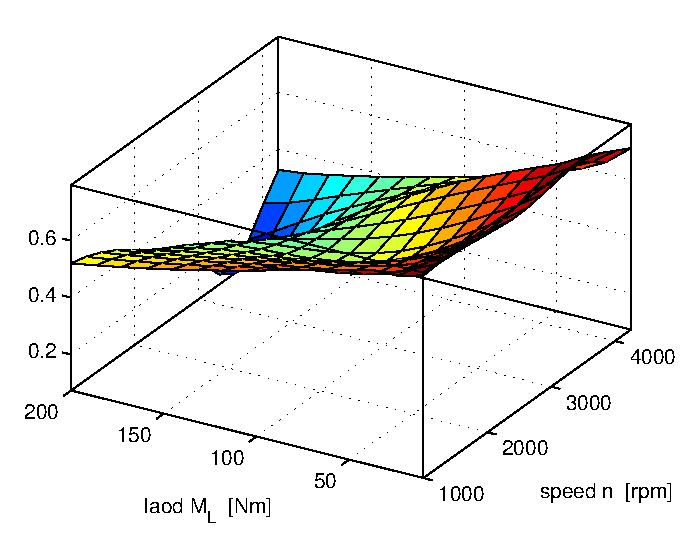
\includegraphics[width=0.75\textwidth]{img/k_surf.eps}
   \caption{Analogy for manifolds}
   \label{img:k_surf}
\end{figure}
			\end{verbatim}
			
			\begin{figure}[ht]
				\centering
				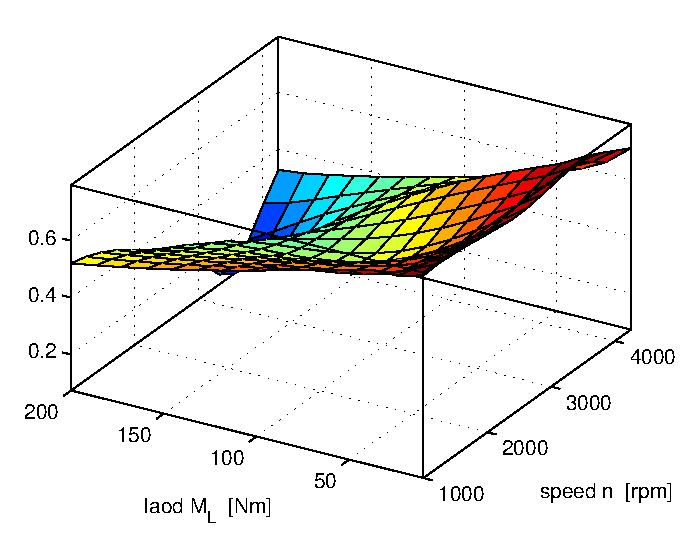
\includegraphics[width=0.75\textwidth]{img/k_surf.eps}
				\caption{Example of a figure.}
				\label{img:k_surf}
			\end{figure}
